\documentclass[10pt]{article}
\usepackage[OT4]{fontenc}
\newtheorem{define}{Definition}
\usepackage[utf8]{inputenc}
\usepackage{bm}
%\newcommand{\Z}{{\mathbb{Z}}}
%\usepackage{psfig}
\usepackage{amsfonts}
\usepackage{amssymb}
\usepackage{graphicx} 
\usepackage{float}
\usepackage{amsfonts}
\usepackage{amsmath}
\usepackage{hyperref}

\setcounter{tocdepth}{4}
\setcounter{secnumdepth}{4}

\oddsidemargin=0.15in
\evensidemargin=0.15in
\topmargin=-.5in
\textheight=9in
\textwidth=6.25in

\begin{document}
%--------------
%% preamble.tex
%% this should be included with a command like
%% %--------------
%% preamble.tex
%% this should be included with a command like
%% %--------------
%% preamble.tex
%% this should be included with a command like
%% \input{preamble.tex}
%% \lecture{1}{September 19, 2012 }{Aleksander Madry}{name of poor scribe}
% % Template based on Dan Spielman's template

\hbadness=10000
\vbadness=10000

\setlength{\oddsidemargin}{.25in}
\setlength{\evensidemargin}{.25in}
\setlength{\textwidth}{6in}
\setlength{\topmargin}{-0.4in}
\setlength{\textheight}{8.5in}


\newcommand{\handout}[5]{
   %\renewcommand{\thepage}{#1-\arabic{page}}
   \noindent
   \begin{center}
   \framebox{
      \vbox{
    \hbox to 5.78in { {\bf Intelligent Data Analysis}
     	 \hfill #2 }
       \vspace{4mm}
       \hbox to 5.78in { {\Large \hfill #5  \hfill} }
       \vspace{2mm}
       \hbox to 5.78in { {\it #3 \hfill} }
       \vspace{0.5mm}
       \hbox to 5.78in { {\it #4 \hfill} }
       
      }
   }
   \end{center}
   \vspace*{4mm}
}

\newcommand{\lecture}[4]{\handout{#1}{#2}{Lecturer:
#3}{Scribes: #4}{Lecture #1}}

\newcommand{\homework}[4]{\handout{#1}{#2}{Professor: #3}{Students: #4}{Homework #1}}
%% usage:
%% \lecture{1}{September 19, 2012 }{Aleksander Madry}{name of poor scribe}


\newtheorem{theorem}{Theorem}
\newtheorem{corollary}[theorem]{Corollary}
\newtheorem{lemma}[theorem]{Lemma}
\newtheorem{observation}[theorem]{Observation}
\newtheorem{proposition}[theorem]{Proposition}
\newtheorem{definition}[theorem]{Definition}
\newtheorem{claim}[theorem]{Claim}
\newtheorem{fact}[theorem]{Fact}
\newtheorem{assumption}[theorem]{Assumption}

%%\newcommand{\qed}{\rule{7pt}{7pt}}
\newcommand{\dis}{\mathop{\mbox{\rm d}}\nolimits}
\newcommand{\per}{\mathop{\mbox{\rm per}}\nolimits}
\newcommand{\area}{\mathop{\mbox{\rm area}}\nolimits}
\newcommand{\cw}{\mathop{\rm cw}\nolimits}
\newcommand{\ccw}{\mathop{\rm ccw}\nolimits}
\newcommand{\DIST}{\mathop{\mbox{\rm DIST}}\nolimits}
\newcommand{\OP}{\mathop{\mbox{\it OP}}\nolimits}
\newcommand{\OPprime}{\mathop{\mbox{\it OP}^{\,\prime}}\nolimits}
\newcommand{\ihat}{\hat{\imath}}
\newcommand{\jhat}{\hat{\jmath}}
\newcommand{\abs}[1]{\mathify{\left| #1 \right|}}

%%\newenvironment{proof}{\noindent{\bf Proof}\hspace*{1em}}{\qed\bigskip}
\newenvironment{proof-sketch}{\noindent{\bf Sketch of Proof}\hspace*{1em}}{\qed\bigskip}
\newenvironment{proof-idea}{\noindent{\bf Proof Idea}\hspace*{1em}}{\qed\bigskip}
\newenvironment{proof-of-lemma}[1]{\noindent{\bf Proof of Lemma #1}\hspace*{1em}}{\qed\bigskip}
\newenvironment{proof-attempt}{\noindent{\bf Proof Attempt}\hspace*{1em}}{\qed\bigskip}
\newenvironment{proofof}[1]{\noindent{\bf Proof}
of #1:\hspace*{1em}}{\qed\bigskip}
\newenvironment{remark}{\noindent{\bf Remark}\hspace*{1em}}{\bigskip}

% \makeatletter
% \@addtoreset{figure}{section}
% \@addtoreset{table}{section}
% \@addtoreset{equation}{section}
% \makeatother

\newcommand{\FOR}{{\bf for}}
\newcommand{\TO}{{\bf to}}
\newcommand{\DO}{{\bf do}}
\newcommand{\WHILE}{{\bf while}}
\newcommand{\AND}{{\bf and}}
\newcommand{\IF}{{\bf if}}
\newcommand{\THEN}{{\bf then}}
\newcommand{\ELSE}{{\bf else}}

% \renewcommand{\thefigure}{\thesection.\arabic{figure}}
% \renewcommand{\thetable}{\thesection.\arabic{table}}
% \renewcommand{\theequation}{\thesection.\arabic{equation}}

\makeatletter
\def\fnum@figure{{\bf Figure \thefigure}}
\def\fnum@table{{\bf Table \thetable}}
\long\def\@mycaption#1[#2]#3{\addcontentsline{\csname
  ext@#1\endcsname}{#1}{\protect\numberline{\csname 
  the#1\endcsname}{\ignorespaces #2}}\par
  \begingroup
    \@parboxrestore
    \small
    \@makecaption{\csname fnum@#1\endcsname}{\ignorespaces #3}\par
  \endgroup}
\def\mycaption{\refstepcounter\@captype \@dblarg{\@mycaption\@captype}}
\makeatother

\newcommand{\figcaption}[1]{\mycaption[]{#1}}
\newcommand{\tabcaption}[1]{\mycaption[]{#1}}
\newcommand{\head}[1]{\chapter[Lecture \##1]{}}
\newcommand{\mathify}[1]{\ifmmode{#1}\else\mbox{$#1$}\fi}
%\renewcommand{\Pr}[1]{\mathify{\mbox{Pr}\left[#1\right]}}
%\newcommand{\Exp}[1]{\mathify{\mbox{Exp}\left[#1\right]}}
\newcommand{\bigO}O
\newcommand{\set}[1]{\mathify{\left\{ #1 \right\}}}
\def\half{\frac{1}{2}}

\newcommand{\fig}[4]{
        \begin{figure}
        \setlength{\epsfysize}{#2}
        \vspace{3mm}
        \centerline{\epsfbox{#4}}
        \caption{#3} \label{#1}
        \end{figure}
        }

\newcommand{\ord}{{\rm ord}}

\providecommand{\norm}[1]{\lVert #1 \rVert}
\newcommand{\embed}{{\rm Embed}}
\newcommand{\qembed}{\mbox{$q$-Embed}}
\newcommand{\calh}{{\cal H}}
\newcommand{\lp}{{\rm LP}}

%% \lecture{1}{September 19, 2012 }{Aleksander Madry}{name of poor scribe}
% % Template based on Dan Spielman's template

\hbadness=10000
\vbadness=10000

\setlength{\oddsidemargin}{.25in}
\setlength{\evensidemargin}{.25in}
\setlength{\textwidth}{6in}
\setlength{\topmargin}{-0.4in}
\setlength{\textheight}{8.5in}


\newcommand{\handout}[5]{
   %\renewcommand{\thepage}{#1-\arabic{page}}
   \noindent
   \begin{center}
   \framebox{
      \vbox{
    \hbox to 5.78in { {\bf Intelligent Data Analysis}
     	 \hfill #2 }
       \vspace{4mm}
       \hbox to 5.78in { {\Large \hfill #5  \hfill} }
       \vspace{2mm}
       \hbox to 5.78in { {\it #3 \hfill} }
       \vspace{0.5mm}
       \hbox to 5.78in { {\it #4 \hfill} }
       
      }
   }
   \end{center}
   \vspace*{4mm}
}

\newcommand{\lecture}[4]{\handout{#1}{#2}{Lecturer:
#3}{Scribes: #4}{Lecture #1}}

\newcommand{\homework}[4]{\handout{#1}{#2}{Professor: #3}{Students: #4}{Homework #1}}
%% usage:
%% \lecture{1}{September 19, 2012 }{Aleksander Madry}{name of poor scribe}


\newtheorem{theorem}{Theorem}
\newtheorem{corollary}[theorem]{Corollary}
\newtheorem{lemma}[theorem]{Lemma}
\newtheorem{observation}[theorem]{Observation}
\newtheorem{proposition}[theorem]{Proposition}
\newtheorem{definition}[theorem]{Definition}
\newtheorem{claim}[theorem]{Claim}
\newtheorem{fact}[theorem]{Fact}
\newtheorem{assumption}[theorem]{Assumption}

%%\newcommand{\qed}{\rule{7pt}{7pt}}
\newcommand{\dis}{\mathop{\mbox{\rm d}}\nolimits}
\newcommand{\per}{\mathop{\mbox{\rm per}}\nolimits}
\newcommand{\area}{\mathop{\mbox{\rm area}}\nolimits}
\newcommand{\cw}{\mathop{\rm cw}\nolimits}
\newcommand{\ccw}{\mathop{\rm ccw}\nolimits}
\newcommand{\DIST}{\mathop{\mbox{\rm DIST}}\nolimits}
\newcommand{\OP}{\mathop{\mbox{\it OP}}\nolimits}
\newcommand{\OPprime}{\mathop{\mbox{\it OP}^{\,\prime}}\nolimits}
\newcommand{\ihat}{\hat{\imath}}
\newcommand{\jhat}{\hat{\jmath}}
\newcommand{\abs}[1]{\mathify{\left| #1 \right|}}

%%\newenvironment{proof}{\noindent{\bf Proof}\hspace*{1em}}{\qed\bigskip}
\newenvironment{proof-sketch}{\noindent{\bf Sketch of Proof}\hspace*{1em}}{\qed\bigskip}
\newenvironment{proof-idea}{\noindent{\bf Proof Idea}\hspace*{1em}}{\qed\bigskip}
\newenvironment{proof-of-lemma}[1]{\noindent{\bf Proof of Lemma #1}\hspace*{1em}}{\qed\bigskip}
\newenvironment{proof-attempt}{\noindent{\bf Proof Attempt}\hspace*{1em}}{\qed\bigskip}
\newenvironment{proofof}[1]{\noindent{\bf Proof}
of #1:\hspace*{1em}}{\qed\bigskip}
\newenvironment{remark}{\noindent{\bf Remark}\hspace*{1em}}{\bigskip}

% \makeatletter
% \@addtoreset{figure}{section}
% \@addtoreset{table}{section}
% \@addtoreset{equation}{section}
% \makeatother

\newcommand{\FOR}{{\bf for}}
\newcommand{\TO}{{\bf to}}
\newcommand{\DO}{{\bf do}}
\newcommand{\WHILE}{{\bf while}}
\newcommand{\AND}{{\bf and}}
\newcommand{\IF}{{\bf if}}
\newcommand{\THEN}{{\bf then}}
\newcommand{\ELSE}{{\bf else}}

% \renewcommand{\thefigure}{\thesection.\arabic{figure}}
% \renewcommand{\thetable}{\thesection.\arabic{table}}
% \renewcommand{\theequation}{\thesection.\arabic{equation}}

\makeatletter
\def\fnum@figure{{\bf Figure \thefigure}}
\def\fnum@table{{\bf Table \thetable}}
\long\def\@mycaption#1[#2]#3{\addcontentsline{\csname
  ext@#1\endcsname}{#1}{\protect\numberline{\csname 
  the#1\endcsname}{\ignorespaces #2}}\par
  \begingroup
    \@parboxrestore
    \small
    \@makecaption{\csname fnum@#1\endcsname}{\ignorespaces #3}\par
  \endgroup}
\def\mycaption{\refstepcounter\@captype \@dblarg{\@mycaption\@captype}}
\makeatother

\newcommand{\figcaption}[1]{\mycaption[]{#1}}
\newcommand{\tabcaption}[1]{\mycaption[]{#1}}
\newcommand{\head}[1]{\chapter[Lecture \##1]{}}
\newcommand{\mathify}[1]{\ifmmode{#1}\else\mbox{$#1$}\fi}
%\renewcommand{\Pr}[1]{\mathify{\mbox{Pr}\left[#1\right]}}
%\newcommand{\Exp}[1]{\mathify{\mbox{Exp}\left[#1\right]}}
\newcommand{\bigO}O
\newcommand{\set}[1]{\mathify{\left\{ #1 \right\}}}
\def\half{\frac{1}{2}}

\newcommand{\fig}[4]{
        \begin{figure}
        \setlength{\epsfysize}{#2}
        \vspace{3mm}
        \centerline{\epsfbox{#4}}
        \caption{#3} \label{#1}
        \end{figure}
        }

\newcommand{\ord}{{\rm ord}}

\providecommand{\norm}[1]{\lVert #1 \rVert}
\newcommand{\embed}{{\rm Embed}}
\newcommand{\qembed}{\mbox{$q$-Embed}}
\newcommand{\calh}{{\cal H}}
\newcommand{\lp}{{\rm LP}}

%% \lecture{1}{September 19, 2012 }{Aleksander Madry}{name of poor scribe}
% % Template based on Dan Spielman's template

\hbadness=10000
\vbadness=10000

\setlength{\oddsidemargin}{.25in}
\setlength{\evensidemargin}{.25in}
\setlength{\textwidth}{6in}
\setlength{\topmargin}{-0.4in}
\setlength{\textheight}{8.5in}


\newcommand{\handout}[5]{
   %\renewcommand{\thepage}{#1-\arabic{page}}
   \noindent
   \begin{center}
   \framebox{
      \vbox{
    \hbox to 5.78in { {\bf Intelligent Data Analysis}
     	 \hfill #2 }
       \vspace{4mm}
       \hbox to 5.78in { {\Large \hfill #5  \hfill} }
       \vspace{2mm}
       \hbox to 5.78in { {\it #3 \hfill} }
       \vspace{0.5mm}
       \hbox to 5.78in { {\it #4 \hfill} }
       
      }
   }
   \end{center}
   \vspace*{4mm}
}

\newcommand{\lecture}[4]{\handout{#1}{#2}{Lecturer:
#3}{Scribes: #4}{Lecture #1}}

\newcommand{\homework}[4]{\handout{#1}{#2}{Professor: #3}{Students: #4}{Homework #1}}
%% usage:
%% \lecture{1}{September 19, 2012 }{Aleksander Madry}{name of poor scribe}


\newtheorem{theorem}{Theorem}
\newtheorem{corollary}[theorem]{Corollary}
\newtheorem{lemma}[theorem]{Lemma}
\newtheorem{observation}[theorem]{Observation}
\newtheorem{proposition}[theorem]{Proposition}
\newtheorem{definition}[theorem]{Definition}
\newtheorem{claim}[theorem]{Claim}
\newtheorem{fact}[theorem]{Fact}
\newtheorem{assumption}[theorem]{Assumption}

%%\newcommand{\qed}{\rule{7pt}{7pt}}
\newcommand{\dis}{\mathop{\mbox{\rm d}}\nolimits}
\newcommand{\per}{\mathop{\mbox{\rm per}}\nolimits}
\newcommand{\area}{\mathop{\mbox{\rm area}}\nolimits}
\newcommand{\cw}{\mathop{\rm cw}\nolimits}
\newcommand{\ccw}{\mathop{\rm ccw}\nolimits}
\newcommand{\DIST}{\mathop{\mbox{\rm DIST}}\nolimits}
\newcommand{\OP}{\mathop{\mbox{\it OP}}\nolimits}
\newcommand{\OPprime}{\mathop{\mbox{\it OP}^{\,\prime}}\nolimits}
\newcommand{\ihat}{\hat{\imath}}
\newcommand{\jhat}{\hat{\jmath}}
\newcommand{\abs}[1]{\mathify{\left| #1 \right|}}

%%\newenvironment{proof}{\noindent{\bf Proof}\hspace*{1em}}{\qed\bigskip}
\newenvironment{proof-sketch}{\noindent{\bf Sketch of Proof}\hspace*{1em}}{\qed\bigskip}
\newenvironment{proof-idea}{\noindent{\bf Proof Idea}\hspace*{1em}}{\qed\bigskip}
\newenvironment{proof-of-lemma}[1]{\noindent{\bf Proof of Lemma #1}\hspace*{1em}}{\qed\bigskip}
\newenvironment{proof-attempt}{\noindent{\bf Proof Attempt}\hspace*{1em}}{\qed\bigskip}
\newenvironment{proofof}[1]{\noindent{\bf Proof}
of #1:\hspace*{1em}}{\qed\bigskip}
\newenvironment{remark}{\noindent{\bf Remark}\hspace*{1em}}{\bigskip}

% \makeatletter
% \@addtoreset{figure}{section}
% \@addtoreset{table}{section}
% \@addtoreset{equation}{section}
% \makeatother

\newcommand{\FOR}{{\bf for}}
\newcommand{\TO}{{\bf to}}
\newcommand{\DO}{{\bf do}}
\newcommand{\WHILE}{{\bf while}}
\newcommand{\AND}{{\bf and}}
\newcommand{\IF}{{\bf if}}
\newcommand{\THEN}{{\bf then}}
\newcommand{\ELSE}{{\bf else}}

% \renewcommand{\thefigure}{\thesection.\arabic{figure}}
% \renewcommand{\thetable}{\thesection.\arabic{table}}
% \renewcommand{\theequation}{\thesection.\arabic{equation}}

\makeatletter
\def\fnum@figure{{\bf Figure \thefigure}}
\def\fnum@table{{\bf Table \thetable}}
\long\def\@mycaption#1[#2]#3{\addcontentsline{\csname
  ext@#1\endcsname}{#1}{\protect\numberline{\csname 
  the#1\endcsname}{\ignorespaces #2}}\par
  \begingroup
    \@parboxrestore
    \small
    \@makecaption{\csname fnum@#1\endcsname}{\ignorespaces #3}\par
  \endgroup}
\def\mycaption{\refstepcounter\@captype \@dblarg{\@mycaption\@captype}}
\makeatother

\newcommand{\figcaption}[1]{\mycaption[]{#1}}
\newcommand{\tabcaption}[1]{\mycaption[]{#1}}
\newcommand{\head}[1]{\chapter[Lecture \##1]{}}
\newcommand{\mathify}[1]{\ifmmode{#1}\else\mbox{$#1$}\fi}
%\renewcommand{\Pr}[1]{\mathify{\mbox{Pr}\left[#1\right]}}
%\newcommand{\Exp}[1]{\mathify{\mbox{Exp}\left[#1\right]}}
\newcommand{\bigO}O
\newcommand{\set}[1]{\mathify{\left\{ #1 \right\}}}
\def\half{\frac{1}{2}}

\newcommand{\fig}[4]{
        \begin{figure}
        \setlength{\epsfysize}{#2}
        \vspace{3mm}
        \centerline{\epsfbox{#4}}
        \caption{#3} \label{#1}
        \end{figure}
        }

\newcommand{\ord}{{\rm ord}}

\providecommand{\norm}[1]{\lVert #1 \rVert}
\newcommand{\embed}{{\rm Embed}}
\newcommand{\qembed}{\mbox{$q$-Embed}}
\newcommand{\calh}{{\cal H}}
\newcommand{\lp}{{\rm LP}}



\homework{number}{date, 2016}{Arminda Moreno Díaz}{Jose Luis Contreras Santos, Antonio Javier González Ferrer and Alejandro González Pérez}

\pagenumbering{gobble}
\tableofcontents

\newpage
\pagenumbering{arabic}

\section{Analysis of the dataset}


\section{Regression}

\subsection{Introduction}
\paragraph*{}
The aim of this section is to use linear regression to model and predict a wine's quality based on its physicochemical attributes. To do this, we will consider the variable `quality` as a continuous variable ranging from 0 to 10. It is worth noting, however, that this variable is originally a categorical one which can only take one of the 11 integer values comprised between 0 and 10. Therefore, as predictions will be continuous, many of them will most likely be slightly off due to this discrepancy. This should not pose a problem,  as the usual error metrics, such as RMSE, can be obtained anyways.

\subsection{Training and test dataset}

\paragraph*{}
The data science pipeline often\footnote{Some statistical learning models are robust enough to do not need this division. They can infer the behavior of the whole population from a sample if some statistical hypothesis are fulfilled.} needs to split the original dataset into two smaller pieces: the train and test datasets. If we only evaluate our models in the same dataset, the results will be overestimated (aka overfitting). To provide honest assessments of the performance of the predictive models, we will need to validate the models using a test dataset, a partition that has not been used to build the models in order to avoid bias. 

\paragraph*{}
In this case, the test dataset consists of the 20\% of the original data (1300 observations) and the training dataset is composed of 5196 data points.

\subsection{Model fitting}
After splitting the data in training and test sets, the training set was used to fit a linear regression model. At first, all variables were used as explanatory variables for the model:

\begin{equation*}
\begin{aligned}	
(1) \ \ \ \  \ \ \ \ \ \ \ \ \ \ \ \ \ \ \ \ \ \ \ \ \ \ \ \ \ \ \hat{y} = \beta_0 + \beta_1*fixed\_acidity + \beta_2*volatile\_acidity 
+ \beta_3*citic\_acid  \\ +\beta_4*residual\_sugar 
+ \ \beta_5*chlorides\\ + \beta_6*free\_sulfur\_dioxide  \\+ \ \beta_7*total\_sulfur\_dioxide   
\\ + \ \beta_8*density + \beta_9*pH  \\+ \ \beta_{10}*sulphates + \beta_{11}*alcohol 	
\end{aligned}
\end{equation*}

However, the marginal coefficient test for each of the variables indicates that the $p$-values for citric acid and chlorides are not low enough to reject the null hypothesis. Thus, we can consider that the contribution of these to the variance of quality is not significantly greater than 0, and so they have been removed from the final model. The resulting linear regression model is described below:

\begin{equation*}
\begin{aligned}	
(2) \ \ \ \  \ \ \ \ \ \ \ \ \ \ \ \ \ \ \ \ \  \hat{y} = 59.58 + 0.0616*fixed\_acidity  -1.275*volatile\_acidity 
+0.04318*residual\_sugar \\
+ \  0.00618*free\_sulfur\_dioxide  - \ 0.00257*total\_sulfur\_dioxide   
\\ - \ 0.5899*density  + \ 0.5068*pH   \\+ 0.7161*sulphates + 0.2637*alcohol
\end{aligned}
\end{equation*}

According to the obtained model, the two variables with the highest influence on quality are `volatile acidity` and `density`, specially the latter. This can be misleading however, as it represents the variation in quality per unit of the input, and the scales of the input variables differ in their order of magnitude. Checking the distribution of $density$, for example, the difference between the maximum and minimum values is lower than 0.03, whereas $total\_sulfur\_dioxide$ has a range of over 400. In any case, some conclusions can be extracted from this output. For example, denser wines tend to have a smaller perceived quality due to the negative coefficient, and, on the contrary, those with higher alcohol contents obtain highger quality perception.

\paragraph*{}
The adjusted R-squared coefficient of the resulting model is rather low, with a value of only 0.29. The regression overall $p$-value, however, is low enough for us to be confident that there exists a relationship between at least part of the input and the output variable, $quality$, performing better than just the simple constant model.

\subsection{Assessing the model: assumptions}

\paragraph*{}
Let us further examine the quality of the linear regression model by checking if the assumptions are met. In particular, we are interested in testing the linearity of the model and if the residuals are independent, normal and have constant variance (LINE conditions).

\begin{figure}[H]
	\centering
	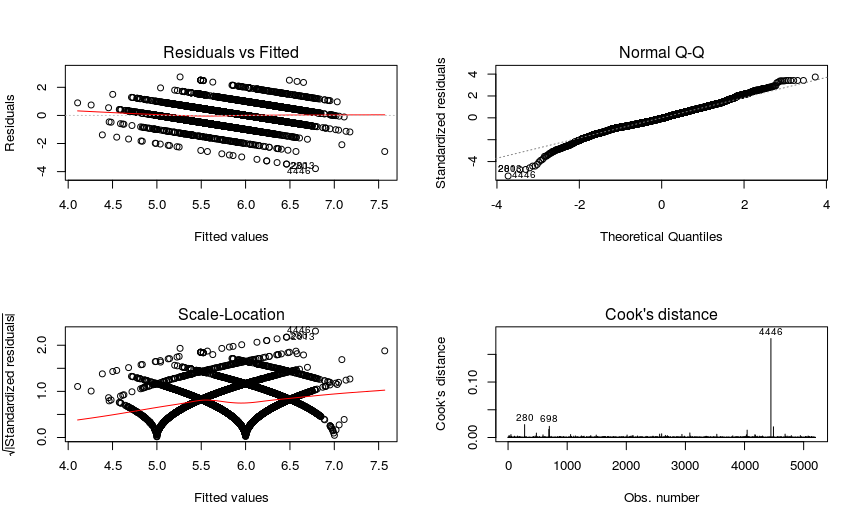
\includegraphics[width=5in]{figures/qqplot.png}
	\caption{Plot diagnostics for the linear regression model} 
	\label{figure:qqplot}
\end{figure}

\paragraph*{}
The conducted tests have different results. First of all, the Rainbow test tests the linear relationship between the response and the linear predictor. The $p$-value is high enough to not reject the null hypothesis (0.4325) but in other datasets this value is close to 1. On the other hand, the Durbin-Watson test returns a high $p$-value (0.7377), sign that there is not enough evidence to reject the null hypothesis of autocorrelation of the residuals. Hence, the residuals can be considered as independent. The results for the Jarque-Bera and Breusch-Pagan tests, however, are not so positive. According to their results, residuals are neither normal nor homoscedastic.

\paragraph*{}
Although the residual plots of Figure \ref{figure:qqplot} are unusual due to the clustering around the integer values, they confirm the previous results. The Normal Q-Q plot is in line with the results of the Jarque-Bera test, showing departures from normality, specially in the first quartiles. From the Cook's distance plot, a significant outlier can be seen, corresponding to observation 4446. Even if we remove this outlier, the statistical assumptions remain the same.
\section{Logistic Regression}

\subsection{Introduction}


\paragraph*{}
Oh!, a wine factory is going to receive a new pack of different wines and they do not have their type labelled (red or white). Ok, don't worry, we can go through each of the wines, look at it color, and label it. But... we would like to do this process automatically.  In the following lines, we will face a classification problem to predict if the wine is red or white, depending on its physicochemical attributes. 

\paragraph*{}
A classification problem relates input variables $x$ to the output variable $y$, but now $y$ can take only discrete values, instead of continuous variables as in regression. When $y$ can only take two discrete, it is called binary classification. We will denote these values as $y \in \{0, 1\}$ in the rest of the report, where $0 \equiv$ white class and $1 \equiv$ red type.

\begin{figure}[H]
	\centering
	
\includegraphics[width=2.5in]{figures/wines.jpg} 
\end{figure}


\subsection{Models}

\paragraph*{}
The equivalent linear regression model in classification is the logistic regression model. This model needs to specify a function such that $p(y=0|\bm{\tilde{X}})$ and $p(y=1|\bm{\tilde{X}})$ are both greater than 0 and sum 1. The logistic function has such properties, defining the following model:

$$ p(y|\bm{\tilde{X}},\bm{\beta}) = \frac{e^{\bm{\beta} \bm{\tilde{X}}}}{1+e^{\bm{\beta} \bm{\tilde{X}}}} $$

If $\beta_i > 0$ then increasing one unit in $x_i$ will increase the probability of a success. If $\beta_i < 0$,
then the probability of success decrease when increasing $x_i$. When $\beta_i = 0$ , $e^0 = 1$, so the odds do not change with $x_i$.

\subsubsection{Full model}

\paragraph*{}
We start by defining a logistic regression model with all the 11 attributes as the predictors. We do not use the `quality`, used in regression, and neither the `type`, used as the target variable $y$:
\begin{equation*}
\begin{aligned}	
(1) \ \ \ \  \ \ \ \ \ \ \ \ \ \ \ \ \ \ \ \ \ \ \ \ \ \ \ \ \ \ logit(\hat{y}) = \beta_0 + \beta_1*fixed\_acidity + \beta_2*volatile\_acidity 
 + \beta_3*citic\_acid  \\ +\beta_4*residual\_sugar 
+ \ \beta_5*chlorides\\ + \beta_6*free\_sulfur\_dioxide  \\+ \ \beta_7*total\_sulfur\_dioxide   
 \\ + \ \beta_8*density + \beta_9*pH  \\+ \ \beta_{10}*sulphates + \beta_{11}*alcohol 	
\end{aligned}
\end{equation*}

At first sight, each of the coefficient has a marginal test which attempts the null hypothesis $H_0$: $\beta_i = 0$, after adjusting the coefficients within the model. That means, it is checked the net effect of each variable and whether should be in the model or not. All the $p$-values are small enough to reject $H_0$ (considering $\alpha = 0.05$) except for `citric\_acid` (0.12) and `sulphates` (0.249). Let us discard these two variables in the further analysis:

\begin{equation*}
\begin{aligned}	
(2) \ \ \ \  \ \ \ \ \ \ \ \ \ \ \ \ \ \ \ \ \  logit(\hat{y}) = \beta_0 + \beta_1*fixed\_acidity + \beta_2*volatile\_acidity 
  +\beta_3*residual\_sugar \\
+ \ \beta_4*chlorides + \beta_5*free\_sulfur\_dioxide  \\+ \ \beta_6*total\_sulfur\_dioxide   
 + \ \beta_7*density \\ + \ \beta_8*pH  +  \beta_{9}*alcohol
\end{aligned}
\end{equation*}

All the marginal tests are now significantly small and the overall fit of the model is high enough ($p = 1$) testing against a Chi-Squared Distribution (pchisq), so we do not have evidence to reject the model in favor of the simple constant model.

\paragraph*{}
We have defined the following metric to validate the correctness of the model based on the confusion matrix of the model. It basically counts the number of correctly classified observations, and it is divided by the total number of examples:

\begin{center}
	accuracy = $\displaystyle \frac{TP+TN}{TP+TN+FP+FN}$
\end{center}

Hence, with the full model we obtain an accuracy of 99\% in both train and test dataset. This can be explained by the fact that the `type` of a wine is clearly defined by a combination of its chemical properties, as expected.

\subsubsection{Simpler models}

\paragraph*{}
Though we obtain a satisfactory accuracy using almost all the variables of the dataset, we would like to find out a simpler model, where just a few attributes were used. This would lead to a more understandable model, easy to interpret and efficient. For instance, we could agree that an optimal model is the one which provides, at least, a 95\% of correct classification.


\paragraph{Constant model}	

Let us start with the simplest model: the constant model. Since we know that the classes are a bit unbalanced, let us start with the model which sets all the labels to 1.

\paragraph*{}
(3) \ \ \ \  $logit(\hat{y}) = 1$

\paragraph*{}
A bit more than 75\% of accuracy just by guessing that all the wines will be red. However, we are not using the chemical information. Let us now include one of the variables to the logistic model. Which one? The one which decreases the most the AIC. The AIC is a measure of the quality of different models, relative to each of the other models. Ideal for model selection.

\paragraph*{}
The function `step` does this task for us: it chooses a model by AIC in a stepwise algorithm. We would use it in the forward direction: tt starts by the simplest constant model, and it tries to achieve the best model up to the full model, previously defined. Since we will go step by step, we will set the number of `steps` manually, to see what happens in each level.

\begin{table}[H]
	\centering
	\begin{tabular}{|l|l|}
		\hline
		\multicolumn{1}{|c|}{\textbf{Variable}} & \multicolumn{1}{c|}{\textbf{AIC}} \\ \hline
		total\_sulfur\_dioxide                  & 2306.6                            \\ \hline
		volatile\_acidity                       & 3522.8                            \\ \hline
		chlorides                               & 3829.2                            \\ \hline
		free\_sulfur\_dioxide                   & 4178.3                            \\ \hline
		fixed\_acidity                          & 4594.0                            \\ \hline
		residual\_sugar                         & 4925.6                            \\ \hline
		density                                 & 4929.1                            \\ \hline
		pH                                      & 5278.9                            \\ \hline
		alcohol                                 & 5836.3                            \\ \hline
	\end{tabular}
		\caption{Comparing logistic regression models using just one predictor}
		\label{table:one-predictor}
\end{table}

\paragraph*{}
Looking at the output in Table \ref{table:one-predictor}, we observe that the best attribute to build a logistic regression with just a single variable is the `total\_sulfur\_dioxide`. The accuracy of the logistic regression variable for both train and test datasets is 92\%! So finally, `type` is almost a matter of sulfur in the liquid. This is, nevertheless, not a surprise, since the most correlated variable with respect to the `type` is also this one (-0.7003).

\paragraph{Two variables model (95\% accuracy)}
Let us include one more variable to the following model and see what happens:

\paragraph*{}
(4) \ \ \ \ $logit(\hat{y}) = \beta_0 + \beta_1*total\_sulfur\_dioxide$

\begin{table}[H]
	\centering
	\begin{tabular}{|l|l|}
		\hline
		\multicolumn{1}{|c|}{\textbf{Variable}} & \multicolumn{1}{c|}{\textbf{AIC}} \\ \hline
		density                                 & 1300.4                            \\ \hline
		volatile\_acidity                       & 1405.4                            \\ \hline
		chlorides                               & 1551.1                            \\ \hline
		fixed\_acidity                          & 1942.0                            \\ \hline
		alcohol                                 & 2072.2                            \\ \hline
		pH                                      & 2142.6                            \\ \hline
		residual\_sugar                         & 2279.6                            \\ \hline
		free\_sulfur\_dioxide                   & 2282.7                            \\ \hline
	\end{tabular}
	\caption{Comparing logistic regression models using two predictors, given `total\_sulfur\_dioxide`.}
	\label{table:two-predictors}
\end{table}


The AIC decays the most with the inclusion of `density`, reaching an accuracy of 95\%. Using just two variables of the dataset, we are just wrong in 58 classifications (21 should have been red, and 37 white) up to a total of 1300 observations.

\paragraph*{}
(5) \ \ \ $logit(\hat{y}) = -782.71663  -0.07262*total\_sulfur\_dioxide +792.08044  *density$

\paragraph*{}
The odds can be interpreted such that the `density` contributes to the probability of getting a red wine (success) while the `total\_sulphur\_dioxide` increases the probability of being classified as a whine type, controlling for the other variable.

\paragraph*{}
We stop here, since the addition of more variables does not significantly increase the accuracy of the model. The following plot summarizes the accuracy of the logistic model with respect the number of variables included in the model, following the stepwise algorithm.


\begin{figure}[H]
	\centering
	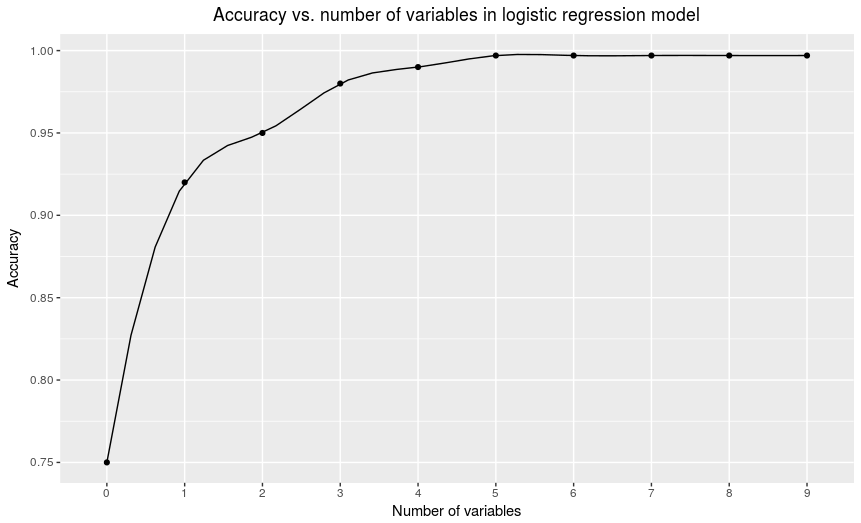
\includegraphics[width=4in]{figures/accuracy-model.png} 
	\caption{Tradeoff between the number of variables used as predictors in the logistic regression and the accuracy.}
	\label{figure:accuracy-model}
\end{figure}

\paragraph{Five variables model (99\% accuracy)}
We can detect in Figure \ref{figure:accuracy-model} that using just 5 variables in the logistic regression mode we achieve the same accuracy (99\%) than using all the 9 variables from the full model (2), getting this final model:
\begin{equation*}
\begin{aligned}	
(6) \ \ \ \ \ \ \ \ \ \ \ \ \ \ \ \ \  \   logit(\hat{y}) = -1.945e^{+3}  -4.375e^{-2}*total\_sulfur\_dioxide + 1.937e^{3}*density \\ \  -7.818e^{-1}*residual\_sugar \\  + \ 2.065*alcohol \\ + \ 7.016*volatile\_acidity
\end{aligned}
\end{equation*}	

Both `total\_sulphur\_dioxide` and `residual\_sugar` decreases the odds of red wine. The probability of being a red wine is less than the probability of being a white whine if you have high values of these two variables. On the other hand, `density`, `alcohol`and `volatile\_acidity` increases the odds of being red type. For instance, when `density` is increased by one unit and all other variables are held constant the odds of $y = 1$ are multiplied by $e^{3}$.

\subsection{Discussion}

\paragraph*{}
After our analysis, we have seen that two different approaches are possible in order to solve our classification problem, introduced at the beginning of this document:

\begin{itemize}
	\item \textbf{Best classification}: In this case, we would like to get the best accuracy as possible. We do not worry in terms of interpretation, but we are looking for the model with less number of parameters that reaches the best accuracy. The model (6) has a 99\% of success using 5 of the original variables. 
	\item \textbf{Simplest explanation}: We are interesting in understanding the data and interpret the parameters of the classification predictors as straightforward as possible, imposing a minimum of accuracy. In our case, the model (5) reaches a 95\% accuracy using just 2 variables, which is very useful to easily describe the model. For instance, we can plot these two variables in the plane:
	
	\begin{figure}[H]
		\centering
		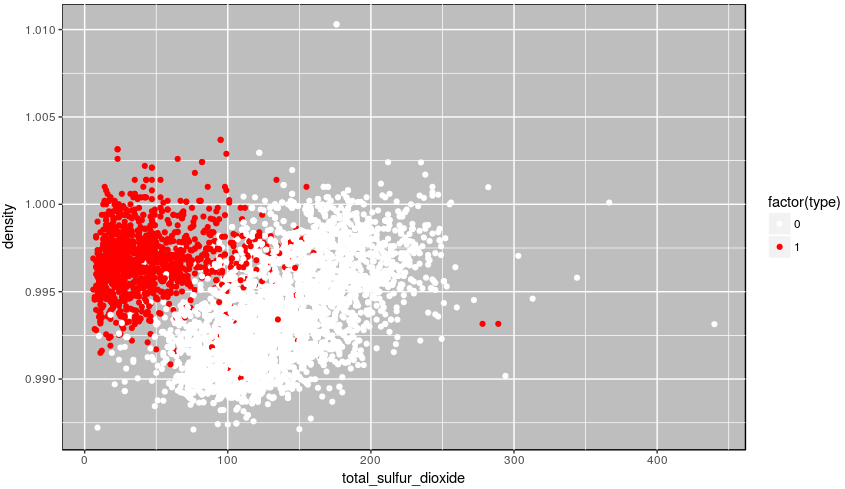
\includegraphics[width=5in]{figures/cluster.png} 
		\caption{Plot total SO$_2$ vs. density and colored by type.}
		\label{figure:cluster}
	\end{figure}
	
	This plot shows the variables `density` and `total\_sulphur\_dioxide` but colored by type. As we can see, it is clear that we have an almost perfect clusters between red and white wines. That is why we are having such a great 95\% accuracy in our simpler model. 
\end{itemize}

\paragraph*{TO (POSSIBLE) DO:}
\begin{itemize}
	\item Analisis de residuos (o comentar porque no los analizamos).
	\item Hacer plot(model) y comentar algo, especialmente del último plot.
	\item Another point.
\end{itemize}
\end{document}




